\documentclass[12pt]{amsart}
\usepackage{amsaddr}
\usepackage{marktext} 
%% Remove draft for real article, put twocolumn for two columns
\usepackage{svmacro}
\usepackage[utf8]{inputenc}
\usepackage[style=alphabetic, backend=biber]{biblatex}
\addbibresource{bibliography.bib}

%% commentary bubble
\newcommand{\SV}[2][]{\sidenote[colback=green!10]{\textbf{SV\xspace #1:} #2}}

%% Title 
\title{ Calculus }
\author{  Mini Exam 2 \\ Second Section \\ \vspace{1cm} Name: \_\_\_\_\_\_\_\_\_\_\_\_\_\_\_\_\_\_\_\_\_\_\_\_\_  
\\ \vspace{1cm} ID: \_\_\_\_\_\_\_\_\_ \\ \vspace{1cm} Score: \_\_\_\_\_\_/ 80}

\date{\today}

\begin{document}

\maketitle


RULES:
\begin{itemize}
	\item You have 30 minutes to complete the exam.
	\item There are 3 questions and 80 points in total.
	\item You can use a non-graphing calculator.
	\item If you need to go to the restroom, please turn in your cellphone before.
	\item If you need hints, 1 hint is worth 3 points.
\end{itemize}


\newpage

\begin{problem}[20 points]
\begin{enumerate}
	\item (10 points) Give a definition of derivative of a function $f(x)$ at $x = a$.
	      \vspace{9cm}
	\item (10 points) Using the definition to compute the derivative of $f(x) = x^3$ at $x = 5$.
	      (You will get 0 point if you use power rule)
	      \vspace{9cm}
\end{enumerate}
\end{problem}

\newpage

\begin{problem}[20 points]
\begin{enumerate}
	\item Find derivative of $\displaystyle f(x) = \frac{x^3 + 4}{x^2 - 4x}$
	      \vspace{10cm}
	\item Find derivative of $\displaystyle f(x) = (4\sin x + 2)(2x^2 - 5)$
	      \vspace{10cm}
	\item Find second derivative of $\displaystyle f(x) = \tan (2x)+ x^2$
	      \vspace{10cm}
	\item Find second derivative of $\displaystyle f(x) = (4x+ 2)(2x^2 - 5)$
	      \vspace{10cm}
\end{enumerate}
\end{problem}

\newpage

\begin{problem}[20 points]
\begin{enumerate}
	\item Find the limit $\displaystyle \lim_{x\to \pi} \frac{x - \pi}{\sin (2x)}$
	      \vspace{10cm}
	\item Find the limit $\displaystyle \lim_{x\to \infty} \frac{e^x}{x^5}$
	      \vspace{10cm}
\end{enumerate}
\end{problem}

\newpage

\begin{problem}[20 points]
The equation $x^4 y^2 + x^2 y^4 = 2$ describes the following picture
\begin{figure}[ht!]
	\begin{center}
		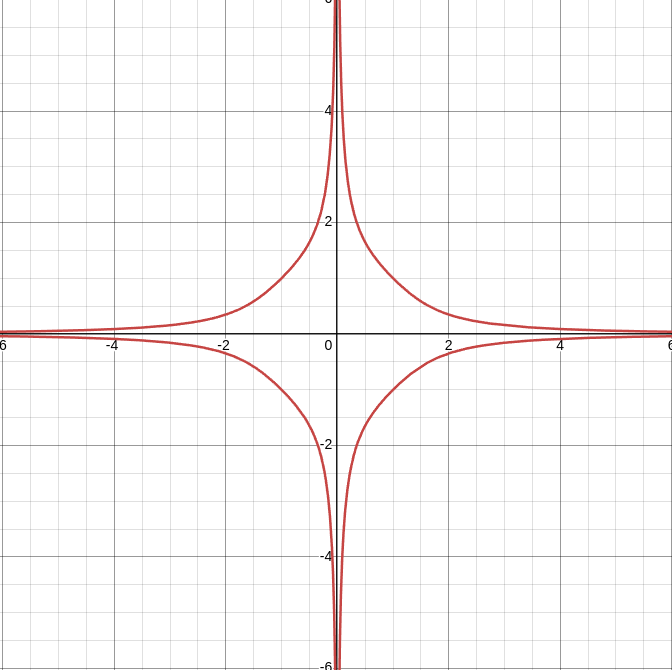
\includegraphics[width = 0.6\linewidth]{fig1.png}
	\end{center}
\end{figure}
\end{problem}
Find the tangent line to this graph at the point $(1,-1)$.


\end{document}
